%!Tex Root = ../main.tex
% ./Packete.tex
% ./Design.tex
% ./Deklarationen.tex
% ./Vorbereitung.tex
% ./Aufgabe1.tex
% ./Aufgabe2.tex
% ./Aufgabe3.tex
% ./Aufgabe4.tex

\section{Appendix}

\begin{frame}[allowframebreaks]{Appendix}{Radix-Komplement}
  \begin{itemize}
    \item Das \alert{Radix-Komplement} (r's Komplement) von einer Zahl y mit $n-$Ziffern mit Radix $b$:
      \begin{equation*}
        b^n-y
      \end{equation*}
    \item Es gibt auch ein \alert{verringertes Radix-Komplement} ((r-1)'s Komplement), und zwar:
      \begin{equation*}
        (b^n-1)-y
      \end{equation*}
      \cite{OnlineRechnerNumerischeKomplemente}
    \item \alert{Komplementärverfahren (engl. Method of complements\cite{MethodComplements2023}):} Subtraktion als Addition berechnen. Beispiele sind: 
            \begin{align*}
                    &\begin{aligned}
                            622_{10} - 451_{10} \text{ ist } 622_{10} + (1000_{10} - 451_{10}) - 1000_{10} &= 622_{10} + (999_{10} - 451_{10} + 1) - 1000_{10}\\
                                                                                                   &= 622_{10} + 549_{10} - 1000_{10}\\
                                                                                                   &= 1171_{10} - 1000_{10} = 171_{10}
                    \end{aligned}\\[0.25cm]
                    &\begin{aligned}
                            110_{2} - 011_{2} \text{ ist } 110_{2} + (1000_{2} - 011_{2}) - 1000_{2} &= 110_{2} + (999_{2} - 011_{2} + 1) - 1000_{2}\\
                                                                                             &= 110_{2} + 101_{2} - 1000_{2}\\ 
                                                                                             &= 1011_{2} - 1000_{2} = 11_{2}
                    \end{aligned}
            \end{align*}
  \end{itemize}
    \begin{Sidenote}
      \begin{itemize}
        \item Das \alert{verringerte Radix-Komplement} kann man leicht erhalten, indem man einfach die Ziffern einer Zahl mit den Ziffern, die man benötigt um $Radix - 1$ zu erhalten, ersetzt. Zum Beispiel, dass verringerte Radix-Komplement für die 2-Ziffern Dezimalzahl $56$ ist $43$. Man kann das \alert{Radix-Komplement} einfach erhalten, indem man Eins zu dem verringerten Radix-Komplement addiert $43+1=44$
        \item Im Dezimalzahlensystem ist das Radix-Komplement auch als \alert{Zehnerkomplement} (10'er Komplement) und das verringerte Radix-Komplement als \alert{Neunerkomplement} (9'er Komplement) bekannt
        \item Im Binärsystem ist das Radix-Komplement als \alert{Zweierkomplement} (2'er Komplement) und das verringerte Radix-Komplement als \alert{Einerkomplement} (1'er Komplement) bekannt. Ein Einerkomplement kann man einfach durch das Umkehren von Bits einer Zahl erhalten. Zweierkomplemente werden in Computern für die Darstellung von negativen Ganzzahlen verwendet
      \end{itemize}
    \end{Sidenote}
\end{frame}

\begin{frame}[allowframebreaks]{Appendix}{Halbaddierer}
  \begin{columns}
    \begin{column}{0.5\textwidth}
      \begin{table}
      \centering
      \begin{tblr}{
          cells = {c},
          hline{3} = {-}{},
      }
        &           & $a$ \\
      $+$ &           & $b$ \\
        & $c_{out}$ & $s$ 
      \end{tblr}
      \end{table}
    \end{column}
    \begin{column}{0.5\textwidth}
      \begin{table}
        \centering
        \begin{tblr}{
          cells = {c, BoxColor},
          row{1} = {SecondaryColor,fg=white},
          vline{3} = {-}{},
        }
        $a$ & $b$ & $c_{out}$ & $s$ \\
         0  &  0  &     0     &  0  \\
         0  &  1  &     0     &  1  \\
         1  &  0  &     0     &  1  \\
         1  &  1  &     1     &  0  
        \end{tblr}
      \end{table}
    \end{column}
  \end{columns}
  \begin{itemize}
    \item der HA kann 2 Inputs zusammenrechen, daher sind die möglichen Outputs $00$, $01$ und $10$
    \item ein HA ist einfach nur die direkte Umsetzung von $a + b = c_{out} \cdot 2^1 + s \cdot 2^0$ nach der obigen Tabelle:
  \end{itemize}
\end{frame}

\begin{frame}[allowframebreaks]{Appendix}{Volladdierer\vspace{0.25cm}}
      % \begin{align*}
      %       a
      %       b
      %     -----
      %     co0s0
      %
      %     ab|co0s0
      %     --+---
      %     00|00
      %     01|01
      %     10|01
      %     11|10
      % \end{align*}
      % \begin{align*}
      %     a
      %     b
      %     ci
      %   ----
      %   co1s1
      %
      %   ciab|co1s1
      %   ---+--
      %   000|00
      %   001|01
      %   010|01
      %   011|10
      %   100|01
      %   101|10
      %   110|10
      %   111|11
      %
      % \end{align*}
  \begin{columns}
    \begin{column}{0.5\textwidth}
      \begin{table}
      \centering
      \begin{tblr}{
        cells = {c},
        hline{4} = {-}{},
      }
          &           & $a$      \\
          &           & $b$      \\
      $+$ &           & $c_{in}$ \\
          & $c_{out}$ & $s$      
      \end{tblr}
      \end{table}
    \end{column}
    \begin{column}{0.5\textwidth}
      \begin{table}
      \centering
      \begin{tblr}{
        cells = {c, BoxColor},
        row{1} = {SecondaryColor, fg=white},
        vline{4} = {-}{},
      }
      $c_{in}$ & $a$ & $b$ & $c_{out}$ & $s$ \\
          0   &  0  &  0  &     0     &  0  \\
          0   &  0  &  1  &     0     &  1  \\
          0   &  1  &  0  &     0     &  1  \\
          0   &  1  &  1  &     1     &  0  \\
          1   &  0  &  0  &     0     &  1  \\
          1   &  0  &  1  &     1     &  0  \\
          1   &  1  &  0  &     1     &  0  \\
          1   &  1  &  1  &     1     &  1  
      \end{tblr}
      \end{table}
    \end{column}
  \end{columns}
  \begin{itemize}
    \item der FA kann 3 Inputs zusammenrechnen, daher sind die möglichen Outputs $00$, $01$ $10$ und $11$
    \item ein FA ist einfach nur die Umsetzung von $a+b+c_{in} = c_{out} \cdot 2^1 + s \cdot 2^0$, ein HA übernimmt $a + b$ und der andere HA übernimmt $s_{a+b} + c_{in}$, wobei es entweder beim ersten HA oder beim zweiten HA die Möglichkeit gibt, dass ein Übertrag entsteht
    \item ob die beiden Überträge am Ende ge$\oplus$rt oder ge$\vee$rt werden spielt keine Rolle, da es sowieso niemals vorkommen kann, dass beide HA einen Übertrag haben
    \begin{itemize}
      \item beim ersten HA kommt es zu einem Übertrag, wenn $a$ und $b$ beide $1$ sind
      \item beim zweiten HA kommt es zu einem Übertrag, wenn $s$ und $c_{in}$ beide $1$ sind
      \item wenn der erste HA einen Übertrag hat, bedeutet es für den zweiten, dass $s = 0$ sein muss es somit beim zweiten zu keinem Übertrag kommen kann. Bei HA kann es nicht vorkommen, dass $c_{out}=1$ und $s=1$
      \item wenn der zweite HA einen Übertrag hat, bedeutet es für den ersten, dass bei diesem $s = 1$ ist und dieser daher keinen Übertrag haben kann
    \end{itemize}
  \end{itemize}
  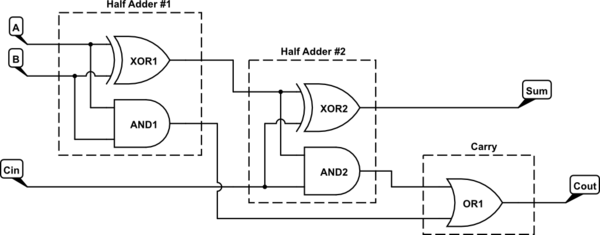
\includegraphics[width=0.8\textwidth, center]{./figures/HA_and_FA.png}
  \begin{itemize}
    \item es spielt bei FA bei der Verwendung keine Rolle, welches der 3 Inputs eigentlich für das Carry vorgesehen ist
  \end{itemize}
\end{frame}

\begin{frame}[allowframebreaks]{Appendix}{4-Bit Addierer}
  \begin{columns}
    \begin{column}{0.3\textwidth}
      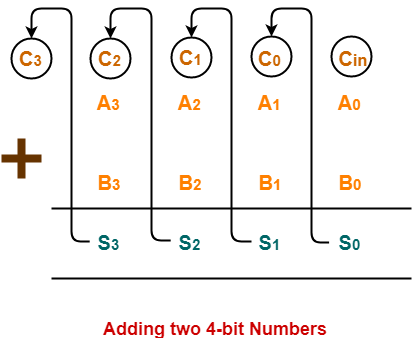
\includegraphics[width=\textwidth, center]{./figures/addition.png}
    \end{column}
    \begin{column}{0.7\textwidth}
      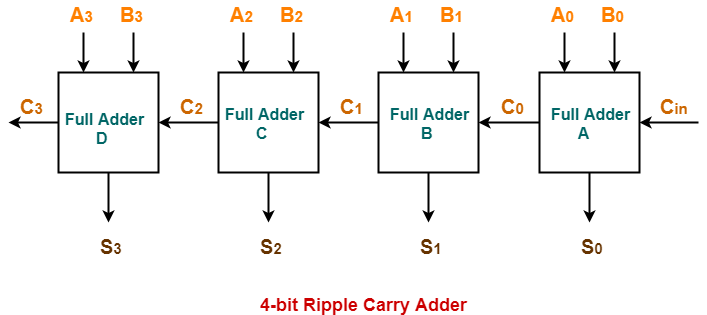
\includegraphics[width=\textwidth, center]{./figures/4_adder_substractor.png}
    \end{column}
  \end{columns}
  \begin{itemize}
    \item FA FA FA HA, wobei man allerdings meistens FA FA FA FA herstellt und das carry vom letzten FA unberührt lässt aber theoretisch Addierer zu größeren Addierern zusammenfügen kann
  \end{itemize}
\end{frame}
